%%%%%%%%%%%%%%%%%%%%%%%%%%%%%%%%%%%%%%%%%
% Arsclassica Article
% LaTeX Template
% Version 1.1 (1/8/17)
%
% This template has been downloaded from:
% http://www.LaTeXTemplates.com
%
% Original author:
% Lorenzo Pantieri (http://www.lorenzopantieri.net) with extensive modifications by:
% Vel (vel@latextemplates.com)
%
% License:
% CC BY-NC-SA 3.0 (http://creativecommons.org/licenses/by-nc-sa/3.0/)
%
%%%%%%%%%%%%%%%%%%%%%%%%%%%%%%%%%%%%%%%%%

%----------------------------------------------------------------------------------------
%	PACKAGES AND OTHER DOCUMENT CONFIGURATIONS
%----------------------------------------------------------------------------------------

\documentclass[
10pt, % Main document font size
a4paper, % Paper type, use 'letterpaper' for US Letter paper
oneside, % One page layout (no page indentation)
%twoside, % Two page layout (page indentation for binding and different headers)
headinclude,footinclude, % Extra spacing for the header and footer
BCOR5mm, % Binding correction
]{scrartcl}

%%%%%%%%%%%%%%%%%%%%%%%%%%%%%%%%%%%%%%%%%
% Arsclassica Article
% Structure Specification File
%
% This file has been downloaded from:
% http://www.LaTeXTemplates.com
%
% Original author:
% Lorenzo Pantieri (http://www.lorenzopantieri.net) with extensive modifications by:
% Vel (vel@latextemplates.com)
%
% License:
% CC BY-NC-SA 3.0 (http://creativecommons.org/licenses/by-nc-sa/3.0/)
%
%%%%%%%%%%%%%%%%%%%%%%%%%%%%%%%%%%%%%%%%%

%----------------------------------------------------------------------------------------
%	REQUIRED PACKAGES
%----------------------------------------------------------------------------------------

\usepackage[
nochapters, % Turn off chapters since this is an article        
beramono, % Use the Bera Mono font for monospaced text (\texttt)
eulermath,% Use the Euler font for mathematics
pdfspacing, % Makes use of pdftex’ letter spacing capabilities via the microtype package
dottedtoc % Dotted lines leading to the page numbers in the table of contents
]{classicthesis} % The layout is based on the Classic Thesis style

\usepackage{arsclassica} % Modifies the Classic Thesis package

\usepackage[T1]{fontenc} % Use 8-bit encoding that has 256 glyphs

\usepackage[utf8]{inputenc} % Required for including letters with accents

\usepackage{graphicx} % Required for including images
\graphicspath{{Figures/}} % Set the default folder for images

\usepackage{enumitem} % Required for manipulating the whitespace between and within lists

\usepackage{lipsum} % Used for inserting dummy 'Lorem ipsum' text into the template

\usepackage{subfig} % Required for creating figures with multiple parts (subfigures)

\usepackage{amsmath,amssymb,amsthm} % For including math equations, theorems, symbols, etc

\usepackage{varioref} % More descriptive referencing

%----------------------------------------------------------------------------------------
%	THEOREM STYLES
%---------------------------------------------------------------------------------------

\theoremstyle{definition} % Define theorem styles here based on the definition style (used for definitions and examples)
\newtheorem{definition}{Definition}

\theoremstyle{plain} % Define theorem styles here based on the plain style (used for theorems, lemmas, propositions)
\newtheorem{theorem}{Theorem}

\theoremstyle{remark} % Define theorem styles here based on the remark style (used for remarks and notes)

%----------------------------------------------------------------------------------------
%	HYPERLINKS
%---------------------------------------------------------------------------------------

\hypersetup{
%draft, % Uncomment to remove all links (useful for printing in black and white)
colorlinks=true, breaklinks=true, bookmarks=true,bookmarksnumbered,
urlcolor=webbrown, linkcolor=RoyalBlue, citecolor=webgreen, % Link colors
pdftitle={}, % PDF title
pdfauthor={\textcopyright}, % PDF Author
pdfsubject={}, % PDF Subject
pdfkeywords={}, % PDF Keywords
pdfcreator={pdfLaTeX}, % PDF Creator
pdfproducer={LaTeX with hyperref and ClassicThesis} % PDF producer
} % Include the structure.tex file which specified the document structure and layout

\hyphenation{Fortran hy-phen-ation} % Specify custom hyphenation points in words with dashes where you would like hyphenation to occur, or alternatively, don't put any dashes in a word to stop hyphenation altogether

\newcommand{\bftheta}{\boldsymbol{\theta}}
\newcommand{\bfmu}{\boldsymbol{\mu}}
\newcommand{\bfalpha}{\boldsymbol{\alpha}}
\newcommand{\bfx}{\boldsymbol{x}}
\newcommand{\bfz}{\boldsymbol{z}}
\newcommand{\bfbeta}{\boldsymbol{\beta}}
\newcommand{\bfpi}{\boldsymbol{\pi}}
\newcommand{\bfe}{\boldsymbol{e}}
\newcommand{\bff}{\boldsymbol{f}}
\DeclareMathOperator{\tr}{tr}

%----------------------------------------------------------------------------------------
%	TITLE AND AUTHOR(S)
%----------------------------------------------------------------------------------------

\title{\normalfont\spacedallcaps{How Many MC Simulations?}} % The article title

%\subtitle{Subtitle} % Uncomment to display a subtitle

\author{\spacedlowsmallcaps{Robert Wolstenholme}} % The article author(s) - author affiliations need to be specified in the AUTHOR AFFILIATIONS block

\date{} % An optional date to appear under the author(s)

%----------------------------------------------------------------------------------------

\begin{document}

%----------------------------------------------------------------------------------------
%	HEADERS
%----------------------------------------------------------------------------------------

\renewcommand{\sectionmark}[1]{\markright{\spacedlowsmallcaps{#1}}} % The header for all pages (oneside) or for even pages (twoside)
%\renewcommand{\subsectionmark}[1]{\markright{\thesubsection~#1}} % Uncomment when using the twoside option - this modifies the header on odd pages
\lehead{\mbox{\llap{\small\thepage\kern1em\color{halfgray} \vline}\color{halfgray}\hspace{0.5em}\rightmark\hfil}} % The header style

\pagestyle{scrheadings} % Enable the headers specified in this block

%----------------------------------------------------------------------------------------
%	TABLE OF CONTENTS & LISTS OF FIGURES AND TABLES
%----------------------------------------------------------------------------------------

\maketitle % Print the title/author/date block

\setcounter{tocdepth}{2} % Set the depth of the table of contents to show sections and subsections only

\tableofcontents % Print the table of contents

\listoffigures % Print the list of figures

\listoftables % Print the list of tables

%----------------------------------------------------------------------------------------
%	ABSTRACT
%----------------------------------------------------------------------------------------

\section*{Abstract} % This section will not appear in the table of contents due to the star (\section*)

When evaluating Baseball matches using Monte Carlo simulations, we would like to know exactly how many simulations it is necessary to perform. For example lets say we wanted to know the probability of the home team beating the away team to 3 decimal places with probability 95\%. Certainly, if we know the distribution of the estimator for our probability (where the variance will depend on the total number of simulations $N$), then its possible to find the value of $N$ necessary for our estimate to be within the given confidence interval. This article is concerned with deriving these distributions along with calculating some realistic examples.

%----------------------------------------------------------------------------------------
%	AUTHOR AFFILIATIONS
%----------------------------------------------------------------------------------------

\let\thefootnote\relax\footnotetext{* \textit{Department of Biology, University of Examples, London, United Kingdom}}

\let\thefootnote\relax\footnotetext{\textsuperscript{1} \textit{Department of Chemistry, University of Examples, London, United Kingdom}}

%----------------------------------------------------------------------------------------

\newpage % Start the article content on the second page, remove this if you have a longer abstract that goes onto the second page

%----------------------------------------------------------------------------------------
%	INTRODUCTION
%----------------------------------------------------------------------------------------

\section{Introduction}

When looking to evaluate an event (e.g. home team beats away team by 0.5), each Monte Carlo simulation is essentially a realisation from a Bernoulli random variable, with values of 1 if the event ocurred or 0 otherwise. The probability of course is unknown. We consider two cases, first where the probability is assumed to be a fixed point, which we call the non-overdispersed case. This arises when all our Monte Carlo simulations come from the same model. We also consider the over-dispersed case, where the probability is assumed to follow a Beta distribution. This arises in our case where we have underlying uncertainty about the skills of the players in our Baseball games. Hence different samples of the players' uncertainties give rise to different models that we Monte Carlo simulate from. Each of these models would have a different associated probability (which we have assumed to be Beta distributed).

In the non-overdispersed case, the only parameter we care about is the total number of simulations for the model $n$ and the value that we should choose to get our event probability estimate within some confidence region. However in the overdispersed case we have two parameters. Again $n$ represents the number of simulations for an individual model but importantly we also have parameter $N$ which represents how many different models we sample, so in total we perform $N \cdot n$ simulations. 

As we have an overhead for creating a model, the time taken in the non-overdispersed case is $n + \delta$ and for the overdispersed case $N \cdot (n +\delta)$ where $\delta$ represents our overhead. Note then in the non-overdispersed case we can directly solve for $n$ when given a confidence interval we wish to be within with some probability. However in the overdispersed case we will instead have two confidence intervals, one for the mean of the probability and another for the variance of the probability. The problem to solve we then be an optimisation, to find the values of $N, n$ that minimise time $N \cdot (n +\delta)$ such that both the mean and variance estimates are within the given confidence intervals.
 
%----------------------------------------------------------------------------------------
%	Non-Overdispersed
%----------------------------------------------------------------------------------------

\section{Non-Overdispersed}
In this case we assume the following model. Let our event be represented by random variable $X$ such that
$$ X \sim Bernoulli(p) $$
where $p$ is a fixed point.

\subsection{Estimator}
Consider $n$ iid random variables with the same distribution as $X$ (representing our Monte Carlo simulations) $X_1, \dots, X_n$. Then we use the following estimator
$$ \hat{P} = \frac{1}{n} \sum_{i=1}^n X_i $$
which by the central limit theroem (CLT) has the following distribution as $n \rightarrow \infty$,
$$ \hat{P} \sim \mathcal{N} \left ( \mathbb{E}[X], \frac{var(X)}{n} \right ) = \mathcal{N} \left( p, \frac{p(1-p)}{n} \right)$$

\subsection{Confidence Interval}
Assume we now want to know $\hat{P}$ within some region with a certain probability i.e.
$$ \Pr (\hat{P} \in (p - \gamma, p + \gamma)|n ) = 1 - \epsilon. $$

Given $\epsilon \in [0,1]$ and $\gamma > 0$, we wish to solve the above equation for $n$. Well assuming as in the limit that $\hat{P}$ follows a normal distribution, then we have

$$ \Phi(\frac{\gamma \sqrt{n}}{\sqrt{p(1-p)}}) - \Phi(\frac{-\gamma \sqrt{n}}{\sqrt{p(1-p)}}) = 1 - \epsilon $$

where $\Phi$ is the cdf of a standard normal distribution. Using the symmetry of the normal distribution about $0$,
$$ \Phi(\frac{\gamma \sqrt{n}}{\sqrt{p(1-p)}}) = 1 - \epsilon/2 $$

\subsection{Example}
Let's use the case mentioned in the abstract, where we want to know the event to 3 decimal place with probability 95\%. In this case we have
$$ \epsilon = 0.05 $$
and
$$ \gamma = 0.0005. $$

We must also set a value for the true probability which we take as
$$ p = 0.5. $$

Plugging into our equation we get
$$ \Phi(\frac{0.0005 \sqrt{n}}{0.5}) = 0.975 $$

$$ \Rightarrow n \approx 3841600 $$

where we used $\Phi^{-1}(0.975) = 1.96$.

This says we need roughly $4,000,000$ simulations to get the desired level of accuracy.


%----------------------------------------------------------------------------------------
%	Overdispersed
%----------------------------------------------------------------------------------------

\section{Overdispersed}
The overdispersed version is a lot more complex than the non-overdispersed version. The model again assumes that our event is represented by random variable $X$ such that
$$ X \sim Bernoulli(P) $$
but in this case $P$ is also a random variable
$$ P \sim Beta(\alpha, \beta). $$

The reason we do this is because as mentioned before, our player skills form a large multivariate normal distribution. Hence to perform our Monte Carlo simulations we must first sample the skills (which we can think of as like sampling a $p$ from $P$). Then we can perform our Bernoulli simulations, sampling $x$ from $X | P=p$.

\subsection{Estimator}
First we begin by defining the random variables that we use. Consider

$$ P_i \sim Beta(\alpha, \beta) $$
for $i = 1 \dots N$,

$$ X_{ij} \sim Bernoulli(P_i) $$
for $j = 1 \dots n$ and

$$ Z_i = \sum_{j=1}^n X_{ij} \sim Binomial(n, P_i). $$

Given the $X_{ij}$ and therefore the $Z_i$, we wish to build estimators for 
$$\mathbb{E}[P_i] = \mathbb{E}[P] = \frac{\alpha}{\alpha + \beta}$$ 
and 
$$ var(P_i) = var(P) = \frac{\alpha \beta}{(\alpha + \beta)^2 (\alpha + \beta + 1)}$$
which are simply results from Beta distributions.

\subsubsection{Moments}
To build the estimators we calculate asymptotic distributions for the estimated raw moments of the $Z_i/n$ (where $Z_i$ follow a Beta-Binomial distribution) and combine these together.

The first raw moment estimator is given by
$$ \hat{\mu}_1 = \frac{1}{N} \sum_{i=1}^N \frac{Z_i}{n} \sim \mathcal{N} \left( \frac{\mathbb{E}[Z_i]}{n}, \frac{var(Z_i)}{Nn^2} \right )$$

as $N \rightarrow \infty$ by the CLT. Using the fact that $Z_i$ is Beta-Binomial distributed we know the moment generating function is the generalised hypergeometric function

$$ M(t) = _2F_1(-n, \alpha; \alpha + \beta; 1 - \exp(t)) $$

and therefore

$$ m_k(\alpha, \beta, n) = \mathbb{E}[Z_i^k] = M^{(k)}(t)|_{t=0}. $$

This means that they may not be pretty, but we can calculate a fixed form for all the moments of the Beta-Binomial. Hence as $N \rightarrow \infty$,

$$ \hat{\mu}_1 \sim \mathcal{N} \left( \frac{\alpha}{\alpha + \beta}, \frac{m_2(\alpha, \beta, n) - m_1(\alpha, \beta, n)^2}{Nn^2} \right ).$$

The second raw moment estimator is given by
$$ \hat{\mu}_2 = \frac{1}{N} \sum_{i=1}^N \frac{Z_i^2}{n^2} \sim \mathcal{N} \left( \frac{\mathbb{E}[Z_i^2]}{n^2}, \frac{var(Z_i^2)}{Nn^4} \right )$$
as $N \rightarrow \infty$. In our Beta-Binomial moment notation, this can be written

$$ \hat{\mu}_2 \sim \mathcal{N} \left( \frac{m_2(\alpha, \beta, n)}{n^2}, \frac{m_4(\alpha, \beta, n) - m_2(\alpha, \beta, n)^2}{Nn^4} \right ).$$

\subsubsection{Combining}
Now lets see how to combine $\hat{\mu_1}$ and $\hat{\mu_2}$ to get unbiased estimators for $\mathbb{E}[P]$ and $var(P)$ with known asymptotic distributions. The first case is easy as clearly

$$ \mathbb{E}[\hat{\mu}_1] = \mathbb{E}[P] $$
and we know the asymptotic distribution of $\hat{\mu}_1$. Hence we can use the combining function 
$$u(\hat{\mu}_1,\hat{\mu}_2) = \hat{\mu}_1$$ 
as our estimator of $\mathbb{E}[P]$. 

The second case is not so easy but we claim the following is an \textit{asymptotically} unbiased estimator of $var(P)$,

$$ v(\hat{\mu}_1,\hat{\mu}_2) = \frac{n \hat{\mu}_2 - \hat{\mu}_1 - (n-1)\hat{\mu}_1^2}{n-1}$$

We write the important lines of the expansion but not that most of the algebra simplification was done by the Sympy package in Python.

$$ \mathbb{E}[v(\hat{\mu}_1,\hat{\mu}_2)] = \frac{\frac{m_2}{n} - \frac{m_1}{n} - (n-1)[var(\hat{\mu}_1) + \mathbb{E}[\hat{\mu}_1]^2]}{n-1} $$
$$ = \frac{\frac{m_2}{n} - \frac{m_1}{n} - (n-1)(\frac{m_1}{n})^2}{n-1} - \frac{m_2 - m_1}{N n^2} $$
$$ = \frac{\alpha \beta}{(\alpha + \beta)^2(\alpha + \beta +1)} - \frac{m_2 - m_1}{N n^2} $$
$$ = var(P) - \frac{m_2 - m_1}{N n^2} $$

If we expand the second term (without the $N$ term) we find
$$\frac{m_2 - m_1}{n^2} = \frac{n-1}{n} \frac{\alpha(\alpha+1)}{(\alpha + \beta)(\alpha + \beta + 1)} \in (0, 1)$$

where as $\alpha, \beta > 0$ we see the smallest value the term can take is $0$ when $\alpha \rightarrow 0$ and the largest is $1$ when $\beta \rightarrow 0$ and $n \rightarrow \infty$.

Hence we have that
$$ var(P) \in (\mathbb{E}[v], \mathbb{E}[v] + \frac{1}{N}) $$
where we dropped the $\hat{\mu}_1,\hat{\mu}_2$ terms for clearer notation. Hence as $N \rightarrow \infty$, $v$ is an unbiased estimator for $var(P)$.

Note that it may be preferable to define our estimator as
$$ \hat{v} = v + \frac{1}{2N} $$
so that
$$ var(P) \in (\mathbb{E}[\hat{v}] - \frac{1}{2N}, \mathbb{E}[\hat{v}] + \frac{1}{2N}) $$
or equivalantly
$$ \mathbb{E}[\hat{v}] \in (var(P) - \frac{1}{2N}, var(P) + \frac{1}{2N}) $$
a symmetric interval. Of course this is then also asymptotically unbiased and has the same variance as $v$. The real benefit comes however with confidence intervals as now let's say we want to know our estimator $\hat{v}$ is within $var(p)$ with \textit{at least} 95\% probability say. Then we want to find $\gamma$ such that

$$ \Pr(\hat{v} \in (var(P) - \gamma, var(P) + \gamma)) > 95\%. $$

Well we can find (using our asymptotic distribution) $\gamma$ such that,
$$ \Pr(\hat{v} \in (\mathbb{E}[\hat{v}] - \gamma +\frac{1}{2N}, \mathbb{E}[\hat{v}] + \gamma - \frac{1}{2N})) = 95\% $$
and therefore using the fact
$$ \hat{v} > \mathbb{E}[\hat{v}] - \gamma + \frac{1}{2N} > var(P) - \gamma $$
and
$$ \hat{v} < \mathbb{E}[\hat{v}] + \gamma - \frac{1}{2N} < var(P) + \gamma $$

we have
$$ \Pr(\hat{v} \in (var(P) - \gamma, var(P) + \gamma)) > 95\% $$
as required.

\subsection{Confidence Interval}
Calculating confidence interval functions for $\mathbb{E}[P]$ is far easier than $var(P)$, so we split them into separate sections.

\subsubsection{Mean}
We have that
$$ u = \hat{\mu}_1 \sim \mathcal{N} \left( \mathbb{E}[P], \frac{m_2 - m_1^2}{Nn^2} \right ).$$

Assume we wish to know $u$ within some region with a certain probability i.e.

$$ \Pr (u \in (\mathbb{E}[P] - \gamma, \mathbb{E}[P] + \gamma)|N, n ) = 1 - \epsilon. $$

Given $\epsilon \in [0,1]$ and $\gamma > 0$, we wish to solve the above equation for $N$ and $n$. Well assuming as in the limit that $u$ follows a normal distribution, then we have

$$ \Phi \left (\frac{\gamma n \sqrt{N}}{\sqrt{m_2 - m_1^2}} \right ) - \Phi \left ( \frac{-\gamma n \sqrt{N}}{\sqrt{m_2 - m_1^2}} \right ) = 1 - \epsilon $$

where $\Phi$ is the cdf of a standard normal distribution. Using the symmetry of the normal distribution about $0$,
$$ \Phi \left (\frac{\gamma n \sqrt{N}}{\sqrt{m_2 - m_1^2}} \right ) = 1 - \epsilon/2. $$

Alternatively we probably just want to make sure that we are at least 95\% sure we are \textit{within} the given confidence interval, given both parameters $N$ and $n$ can vary i.e.

\begin{equation} \label{eqn.mean_dist} 
\Phi \left (\frac{\gamma n \sqrt{N}}{\sqrt{m_2 - m_1^2}} \right ) > 1 - \epsilon/2.
\end{equation} \label{eqn.mean_dist}

\subsubsection{Variance}
In order to find confidence intervals using $v$ we note that it is actually just the sample variance of $Z_i$ plus a term that goes to zero as $n \rightarrow \infty$. We proceed as follows

$$ v = \frac{n \hat{\mu}_2 - \hat{\mu}_1 - (n-1)\hat{\mu}_1^2}{n-1}$$
$$ = \frac{n}{n-1} (\hat{\mu}_2 - \hat{\mu}_1^2) + \frac{1}{n-1} (\hat{\mu}_1^2 - \hat{\mu}_1)$$
$$ = \frac{n}{n-1} \left [ \frac{1}{N} \sum_{i=1}^N \frac{Z_i^2}{n^2} - \left( \frac{1}{N} \sum_{i=1}^N \frac{Z_i}{n} \right )^2 \right ] + \frac{\hat{\mu}_1^2 - \hat{\mu}_1}{n-1}$$
$$ = \frac{N-1}{Nn(n-1)} \left [ \frac{N \sum_{i=1}^N Z_i^2 - \left( \sum_{i=1}^N Z_i \right )^2}{N(N-1)} \right ] + \frac{\hat{\mu}_1^2 - \hat{\mu}_1}{n-1}$$

The term in square brackets is simply the sample variance of $Z$ written
$$ s^2(Z) = \frac{N \sum_{i=1}^N Z_i^2 - \left( \sum_{i=1}^N Z_i \right )^2}{N(N-1)}. $$

We note when considering the second term that as $\hat{\mu}_1 \in [0,1]$,

$$ 0 < \frac{\hat{\mu}_1^2 - \hat{\mu}_1}{n-1} < \frac{1}{4(n-1)} $$

and so as $n, N \rightarrow \infty$, $v \rightarrow \frac{s^2(Z)}{n^2} $. Its a result \cite{bworld} that asymptotically the sample variance tends to the following

$$ s^2(Z) \rightarrow \mathcal{N} \left (\sigma^2(Z), \frac{\mathbb{E}[(Z - \mathbb{E}[Z])^4] - \sigma^4(Z)}{N} \right )$$

where $\sigma(Z) = \sqrt{\mathbb{E}[Z^2] - \mathbb{E}[Z]^2}$ is the standard deviation of $Z$. So writing using our $\mathbb{E}[Z^k] = m_k$ notation we have

$$ v \rightarrow \mathcal{N} \left ( \frac{m_2 - m_1^2}{n^2}, \frac{m_4 - 4m_3m_1 + 8m_2m_1^2 - 4m_1^4 - m_2^2}{Nn^4} \right )$$
which gives us the asymptotic distriution we require.

A quick sanity check shows that as $n \rightarrow \infty$,
$$ \frac{m_2 - m_1^2}{n^2} = \frac{n \alpha \beta (\alpha + \beta + n)}{n^2 (\alpha + \beta)^2(\alpha + \beta + 1)} \rightarrow \frac{\alpha \beta}{ (\alpha + \beta)^2(\alpha + \beta + 1)} = var(P)$$

as we would expect.

Now, assume we wish to know $v$ within some region with a certain probability i.e.

$$ \Pr (v \in (var(P) - \gamma, var(P) + \gamma)|N, n ) = 1 - \epsilon. $$

Given $\epsilon \in [0,1]$ and $\gamma > 0$, we wish to solve the above equation for $N$ and $n$. Well assuming as in the limit that $v$ follows a normal distribution, then we have using the symmetry of the normal distribution about $0$,

$$ \Phi \left (\frac{\gamma n^2 \sqrt{N}}{\sqrt{m_4 - 4m_3m_1 + 8m_2m_1^2 - 4m_1^4 - m_2^2}}\right ) = 1 - \epsilon/2. $$

where $\Phi$ is the cdf of a standard normal distribution. 

 
Alternatively we probably just want to make sure that we are at least 95\% sure we are \textit{within} the given confidence interval, given both parameters $N$ and $n$ can vary i.e.
\begin{equation} \label{eqn.var_dist}
 \Phi \left (\frac{\gamma n^2 \sqrt{N}}{\sqrt{m_4 - 4m_3m_1 + 8m_2m_1^2 - 4m_1^4 - m_2^2}}\right ) > 1 - \epsilon/2.
 \end{equation}

As we mentioned before, it isn't pretty, but the $m_k$ are simply functions of $\alpha, \beta$ and $n$.

We can now think of equations (\ref{eqn.mean_dist}) and (\ref{eqn.var_dist}) as giving some constraints on our $N$ and $n$ values and we aim to minimise $N (n + \delta)$ subject to those constraints. We may want to add some further constraints i.e. $N > 1000$ and $n > 500$ to make sure the CLT is taking effect and we don't choose some trivially small solution.

\subsection{Example}
\subsubsection{Mean}
Let's again use the case mentioned in the abstract, where we want to know the event to 3 decimal place with \textit{at least} probability 95\%. In this case we have
$$ \epsilon = 0.05 $$
and
$$ \gamma = 0.0005. $$

We must also set values for $\alpha$ and $\beta$, which we take as
$$ \alpha = 0.5 $$
and
$$ \beta = 0.5. $$

Plugging into our moment equations we get
$$ m_1^2 = \frac{n^2}{4} $$
and
$$ m_2 = \frac{n(3n+1)}{8} $$

So
$$ \frac{0.0005 n \sqrt{N}}{(\sqrt{n(3n+1) - 2n^2)/8}} > 1.96 $$
$$ \Rightarrow 8 \cdot 0.0005^2 n^2 N > 1.96^2(n(3n+1) -2n^2 )$$
\begin{equation} \label{eqn.example}
  \Rightarrow \frac{8 \cdot 0.0005^2}{1.96^2} n^2 N - n^2 - n > 0
\end{equation}

where we used $\Phi^{-1}(0.975) = 1.96$. Note that we can rearrange and using
the fact $n, N > 0$, we get

$$ \frac{8 \cdot 0.0005^2}{1.96^2}  N - 1 > \frac{1}{n} $$

which means that $N$ must satisfy

$$ N > \frac{1.96^2}{8 \cdot 0.0005^2} = 1920800 $$

Of course if we use near the minimal value of $N$, it could result in extremely
large $n$ values. If instead we use a few different values of $n$ we can get
corresponding $N$ values necessary to be within the limits.

\begin{table}[hbt]
\caption{Table of $N$ satisfying (\ref{eqn.example}) for different $n$}
\centering
\begin{tabular}{rr}

n & N \\
\midrule
$2$ & $2881200$ \\
$5$ & $2304960$ \\
$10$ & $2112880$ \\
$100$ & $1940008$ \\
$1000$ & $1922720$ \\
$10000$ & $1920992$ \\
\bottomrule
\end{tabular}
\label{tab:label}
\end{table}


Note that despite the fact there isn't that much improvement in simulations as it increases, we expect small $n$ values to require many more simulations to get a decent $var(P)$ estimate. Note also that the $\alpha$ and $\beta$ values chosen may not reflect reality (in this case it gives a much larger variance than we would expect). Practically we want to choose values for these that roughly make sense for a given event. The next table shows simulation numbers for different $\gamma, \alpha, \beta, n$ values.

\begin{table}[hbt]
\caption{Table of $N$ satisfying 95\% confidence interval for different $\gamma, \alpha, \beta, n$}
\centering
\begin{tabular}{rrrrr}

$\gamma$ & $\alpha$ & $\beta$ & $n$ & $N$ \\
\midrule
$0.0005$ & $0.5$ & $0.5$ & $1000$ & $1922720$ \\
$0.0005$ & $5$ & $5$ & $1000$ & $352728$ \\
$0.0005$ & $5$ & $5$ & $100$ & $384160$ \\
$0.0005$ & $50$ & $50$ & $1000$ & $41839$ \\
$0.0005$ & $50$ & $50$ & $100$ & $76071$ \\
$0.005$ & $50$ & $50$ & $100$ & $418$ \\

\bottomrule
\end{tabular}
\label{tab:label}
\end{table}

The above values were calculated using mean\_sims.py. We see that as the values of $\alpha$ and $beta$ increase (i.e. $var(P)$ decreases) the number of simulations $N$ necessary rapidly decreases.

\subsubsection{Variance}
TODO


\section{Results and Discussion}

Reference to Figure~\vref{fig:gallery}. % The \vref command specifies the location of the reference

\begin{figure}[tb]
\centering 
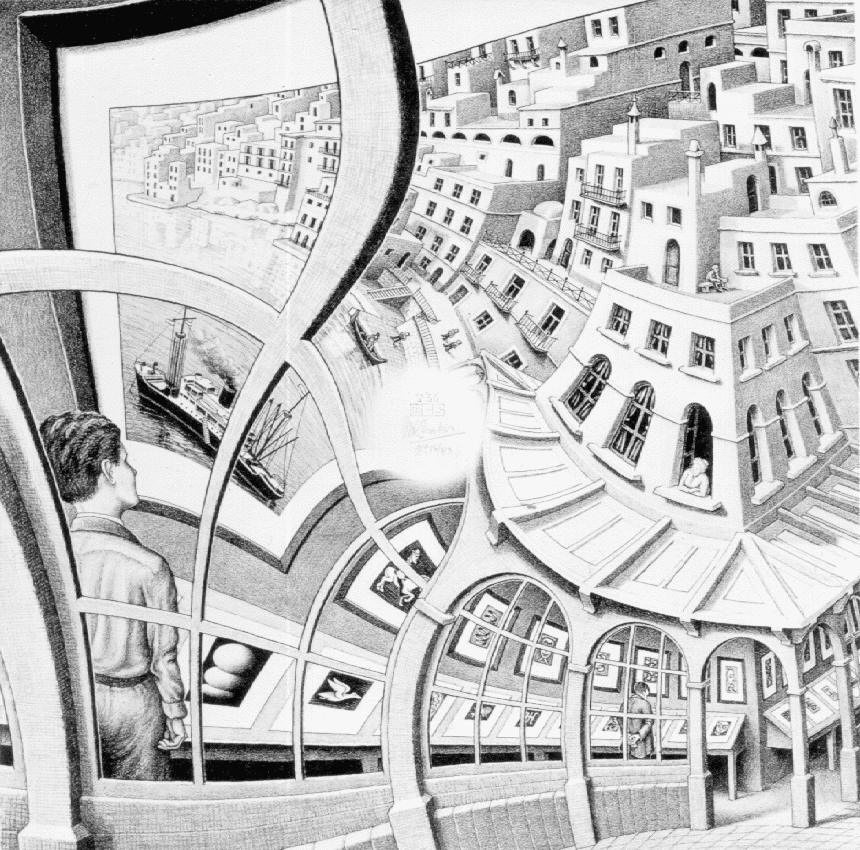
\includegraphics[width=0.5\columnwidth]{GalleriaStampe} 
\caption[An example of a floating figure]{An example of a floating figure (a reproduction from the \emph{Gallery of prints}, M.~Escher,\index{Escher, M.~C.} from \url{http://www.mcescher.com/}).} % The text in the square bracket is the caption for the list of figures while the text in the curly brackets is the figure caption
\label{fig:gallery} 
\end{figure}

\lipsum[10] % Dummy text

%------------------------------------------------

\subsection{Subsection}

\lipsum[11] % Dummy text

\subsubsection{Subsubsection}

\lipsum[12] % Dummy text

\begin{description}
\item[Word] Definition
\item[Concept] Explanation
\item[Idea] Text
\end{description}

\lipsum[12] % Dummy text

\begin{itemize}[noitemsep] % [noitemsep] removes whitespace between the items for a compact look
\item First item in a list
\item Second item in a list
\item Third item in a list
\end{itemize}

\subsubsection{Table}

\lipsum[13] % Dummy text

\begin{table}[hbt]
\caption{Table of Grades}
\centering
\begin{tabular}{llr}
\toprule
\multicolumn{2}{c}{Name} \\
\cmidrule(r){1-2}
First name & Last Name & Grade \\
\midrule
John & Doe & $7.5$ \\
Richard & Miles & $2$ \\
\bottomrule
\end{tabular}
\label{tab:label}
\end{table}

Reference to Table~\vref{tab:label}. % The \vref command specifies the location of the reference

%------------------------------------------------

\subsection{Figure Composed of Subfigures}

Reference the figure composed of multiple subfigures as Figure~\vref{fig:esempio}. Reference one of the subfigures as Figure~\vref{fig:ipsum}. % The \vref command specifies the location of the reference

\lipsum[15-18] % Dummy text

\begin{figure}[tb]
\centering
\subfloat[A city market.]{
\includegraphics[width=.45\columnwidth]{Lorem}} \quad
\subfloat[Forest landscape.]{
\includegraphics[width=.45\columnwidth]{Ipsum}\label{fig:ipsum}} \\
\subfloat[Mountain landscape.]{
\includegraphics[width=.45\columnwidth]{Dolor}} \quad
\subfloat[A tile decoration.]{
\includegraphics[width=.45\columnwidth]{Sit}}
\caption[A number of pictures.]{A number of pictures with no common theme.} % The text in the square bracket is the caption for the list of figures while the text in the curly brackets is the figure caption
\label{fig:esempio}
\end{figure}

%----------------------------------------------------------------------------------------
%	BIBLIOGRAPHY
%----------------------------------------------------------------------------------------

\renewcommand{\refname}{\spacedlowsmallcaps{References}} % For modifying the bibliography heading

\bibliographystyle{unsrt}

\bibliography{sample.bib} % The file containing the bibliography

%----------------------------------------------------------------------------------------

\end{document}
